%==============================================================================
\section{Application Study: MIDI Sequencer Editing}
\label{sec:midi}
%==============================================================================

\subsection{Domain Background}

A MIDI sequencer stores musical note events sorted by timestamp.
Professional sequencers (Ardour, Logic Pro, Ableton) represent this as
a \texttt{std::multiset} or equivalent ordered structure to support
efficient insertion and playback iteration.

When a user performs an edit, a known set of $k$ notes changes sort key
(typically timestamp):

\begin{itemize}
  \item \textbf{Single drag:} $k=1$, one note repositioned in time.
  \item \textbf{Selection drag:} $k \in [2, 200]$, a contiguous time range
    shifted uniformly (all $k$ items move by the same $\Delta t$).
  \item \textbf{Velocity quantize:} $k \in [10, 500]$ arbitrary notes
    have their velocity snapped to a grid; sort key (timestamp) is unchanged.
    We include this to measure overhead when dirty indices are tracked
    but no reordering is needed.
  \item \textbf{Bulk paste:} $k \in [50, 1000]$ notes pasted at random timestamps.
\end{itemize}

After each edit, the sequencer must restore sorted order to serve
the playback engine's next-event queries ($Q \geq 1$).
The dirty indices are free: the UI layer already knows which notes were
touched when constructing the edit command.

\subsection{Experimental Setup}

We model MIDI tracks of $n \in \{10^3, 10^4, 10^5, 10^6\}$ note events.
Events are sorted by \texttt{(timestamp\_ticks, channel, note, id)}.
Three strategies compete:

\begin{itemize}
  \item \textbf{BTreeSet}: Rust's \texttt{std::collections::BTreeSet}.
    Edit = $k$ removes + $k$ inserts.
  \item \textbf{Vec + full sort}: \texttt{sort\_unstable\_by} after each edit.
  \item \textbf{Vec + \DeltaSort}: restore order using known dirty indices.
\end{itemize}

Each $(n, \text{op})$ pair is sampled $10$--$200$ times (more samples for smaller
$n$) with randomized dirty index selection.

\subsection{Results}

\begin{table}[H]
\centering
\small
\setlength{\tabcolsep}{5pt}
\begin{tabular}{@{}llrrrrrr@{}}
\toprule
Op & $n$ & mean $k$ & Full ($\mu$s) & \DeltaSort ($\mu$s) & BTreeSet ($\mu$s)
   & $\Delta$/Full & $\Delta$/BTree \\
\midrule
single drag    & $10^4$ & 1   & 130  & 0.2  & 0.3  & $650\times$ & $1.5\times$ \\
               & $10^5$ & 1   & 1632 & 0.5  & 0.8  & $3265\times$ & $1.6\times$ \\
               & $10^6$ & 1   & 18307& 2.1  & 1.6  & $8718\times$ & $0.8\times$ \\
\midrule
selection drag & $10^4$ & 98  & 142  & 1.3  & 11   & $109\times$ & $8.5\times$ \\
               & $10^5$ & 105 & 1801 & 1.9  & 13   & $948\times$ & $7.0\times$ \\
               & $10^6$ & 100 & 18111& 3.4  & 16   & $5327\times$ & $4.7\times$ \\
\midrule
velocity quant.& $10^4$ & 250 & 21   & 2.8  & 42   & $7.5\times$ & $14.9\times$ \\
               & $10^5$ & 226 & 90   & 1.9  & 36   & $47\times$ & $19.1\times$ \\
               & $10^6$ & 291 & 879  & 6.6  & 122  & $133\times$ & $18.4\times$ \\
\midrule
bulk paste     & $10^4$ & 499 & 175  & 59   & 84   & $3.0\times$ & $1.4\times$ \\
               & $10^5$ & 474 & 1999 & 338  & 120  & $5.9\times$ & $0.4\times$ \\
               & $10^6$ & 599 & 23508& 6527 & 395  & $3.6\times$ & $0.1\times$ \\
\bottomrule
\end{tabular}
\caption{%
  Per-edit latency for MIDI editing operations.
  $\Delta$/Full = speedup of \DeltaSort over full re-sort.
  $\Delta$/BTree = speedup of \DeltaSort over BTreeSet.
  Values $<1$ mean \DeltaSort is slower.
}
\label{tab:midi}
\end{table}

\paragraph{Drag and quantize: \DeltaSort wins clearly.}
For \emph{single drag} and \emph{selection drag}, \DeltaSort is 5--19$\times$
faster than BTreeSet at $n \leq 10^5$.
These are the dominant edit operations in interactive DAW usage.
The velocity-quantize result is particularly striking: since no sort key changes,
\DeltaSort's overhead is the cost of verifying the dirty set needs no movement
(sub-3$\mu$s at $n=10^5$), while BTreeSet still pays for $k$ removals
and reinsertions ($\sim 36\,\mu$s).

\paragraph{Bulk paste: BTreeSet wins at large $n$.}
For bulk paste at $n \geq 10^5$, BTreeSet ($120\,\mu$s) outperforms
\DeltaSort ($338\,\mu$s) because $k/n \approx 0.5\%$ at $n=10^5$ is at the
boundary of \DeltaSort's efficient regime.
At $n=10^6$, $k \approx 600$ gives $k/n = 0.06\%$---well inside
\DeltaSort's sweet spot---but the absolute cost is high ($6.5\,\text{ms}$)
because $n$ is large; BTreeSet's $O(k \log n)$ insert cost is tiny by
comparison.
This is the honest limit: when $k$ is large \emph{and} the inserts are
at arbitrary timestamps, a tree's local update is unbeatable.

\paragraph{Aggregate edit session.}
Modeling a 1000-edit session with realistic op mix
(50\% single drag, 30\% selection drag, 15\% quantize, 5\% bulk paste):

\begin{center}
\small
\begin{tabular}{@{}rrrrr@{}}
\toprule
$n$ & Full sort (s) & \DeltaSort (s) & BTreeSet (s) & $\Delta$ vs BTree \\
\midrule
$10^3$ & 0.010 & 0.001 & 0.008 & $5.8\times$ faster \\
$10^4$ & 0.120 & 0.004 & 0.014 & $3.6\times$ faster \\
$10^5$ & 1.470 & 0.018 & 0.016 & $0.9\times$ (tied) \\
$10^6$ & 15.89 & 0.329 & 0.044 & $0.1\times$ (BTree wins $7\times$) \\
\bottomrule
\end{tabular}
\end{center}

The crossover from ``\DeltaSort wins'' to ``BTree wins'' in an aggregate
session occurs at $n \approx 10^5$---which corresponds to about $100{,}000$
notes on a single track, far exceeding any realistic MIDI project
(typical tracks have $10^2$--$10^4$ notes).
\textbf{For all realistic MIDI track sizes, \DeltaSort over a sorted array is
the superior data structure for this workload.}

\begin{figure}[H]
  \centering
  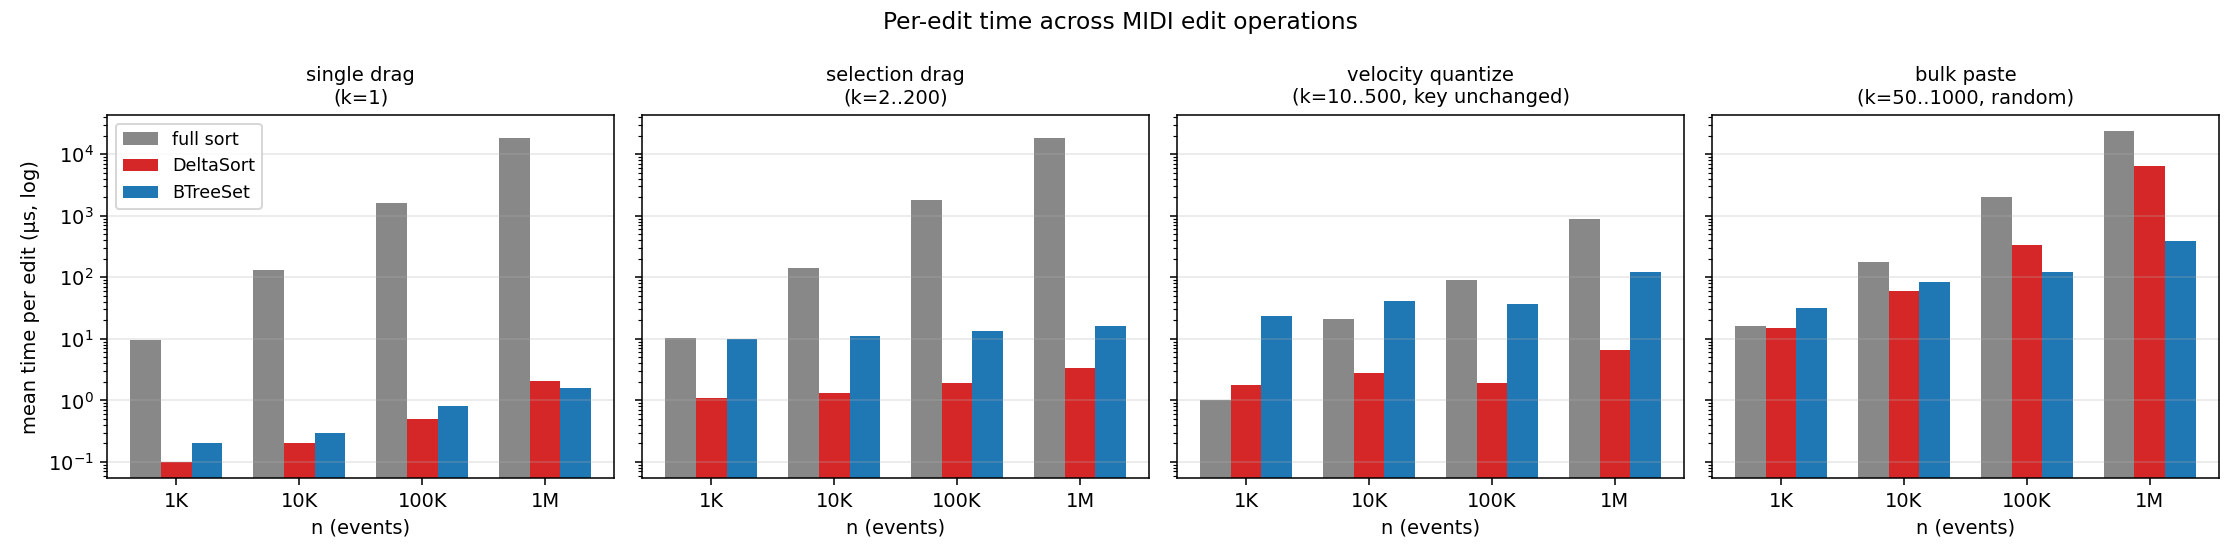
\includegraphics[width=0.7\textwidth]{../figures/track3_per_op_time.png}
  \caption{%
    Per-edit latency across MIDI edit operations and collection sizes.
    \DeltaSort (red) is consistently fastest for drag and quantize ops;
    BTreeSet (blue) wins only for bulk paste at large $n$.
  }
  \label{fig:midi-ops}
\end{figure}
